w\chapter{IMPLEMENTASI}
  Pada bab ini dibahas mengenai implementasi aplikasi sesuai dengan perancangan sistem yang telah dijelaskan sebelumnya. Bahasa pemrograman yang digunakan antara lain PHP, SQL, Javascript.
  
  \section{Lingkungan Implementasi}
  Lingkungan pembangunan dijelaskan pada subbab ini.
  
  
  \subsection{Lingkungan Pembangun Perangkat Keras}
  
  Aplikasi dideploy secara \textit{online}, dalam sebuah \textit{Virtual Private Server} yang di\textit{host} oleh \textit{Digital Ocean}.
  Spesifikasi VPS yang digunakan adalah sebagai berikut :
  
  \begin{enumerate}
  	\item Hardware
		  \begin{enumerate}
		  	\item CPU: Intel(R) Xeon(R) CPU E5-2630L v2 @ 2.40GHz
		  	\item Operating System : 
		  	\item RAM : 512MB
		  	\item Storage Space : 20GB
		  \end{enumerate}
		  
   \item Operating System
	   \begin{enumerate}
	   	\item Architecture : 64bit
	   	\item Kernel Version : Linux 4.4.0-75-generic x86 64
	   	\item OS Version : Ubuntu 16.04.2 LTS Xenial
	   	\end{enumerate}
	   	
	\item Networking Stats
		\begin{enumerate}
			\item Tersambung ke Internet : Ya
			\item IP Publik : Ya
			\item Alamat IP Publik (IPv4) : 188.166.179.2
			\item \textit{Average Download Speed} : 1371 Mbit/s
			\item \textit{Average Upload Speed} : 860.12 Mbit/s
			\item DNS : Google
		\end{enumerate}
		
	\item Domain Stats
		\begin{enumerate}
			\item HTTPS Support : Yes
			\item SSL Certificate issued by : Avast
			\item Domain : https://Lelangapa.com
			\item Testing-purpose subdomain : https://testing.lelangapa.com
			\item Domain issued by : Namecheap
		\end{enumerate}
	
  \end{enumerate}
  
  \subsection{Lingkungan Pembangun Perangkat Lunak}
  Spesifikasi perangkat lunak yang digunakan untuk membuat tugas akhir ini adalah sebagai berikut:
	  \begin{enumerate}
	  \item Google Chrome sebagai media akses aplikasi
	  \item PgAdmin, sebagai Database Management \& Editor
	  \item PHPStorm sebagai IDE utama
	  \item Nano untuk \textit{shell text editor}
	  \item Postman, untuk \textit{debugging} API \textit{calls} dan system tests
	  \item Power Designer untuk alat bantu desain yang berhubungan dengan grafis seperti diagram, \textit{flowchart}, dll.
	  \end{enumerate}
  
\section{Implementasi Antarmuka}
	
    \subsection{Antarmuka Registrasi}
    
    Penjelasan otorisasi terhadap antarmuka A, link yang tersedia dalam antarmuka A, dan penjelasan \textit{exception} jika terjadi masalah baik otorisasi ataupun autentikasi saat mengakses antarmuka ini.
  
      \begin{figure}[H]
        \centering
        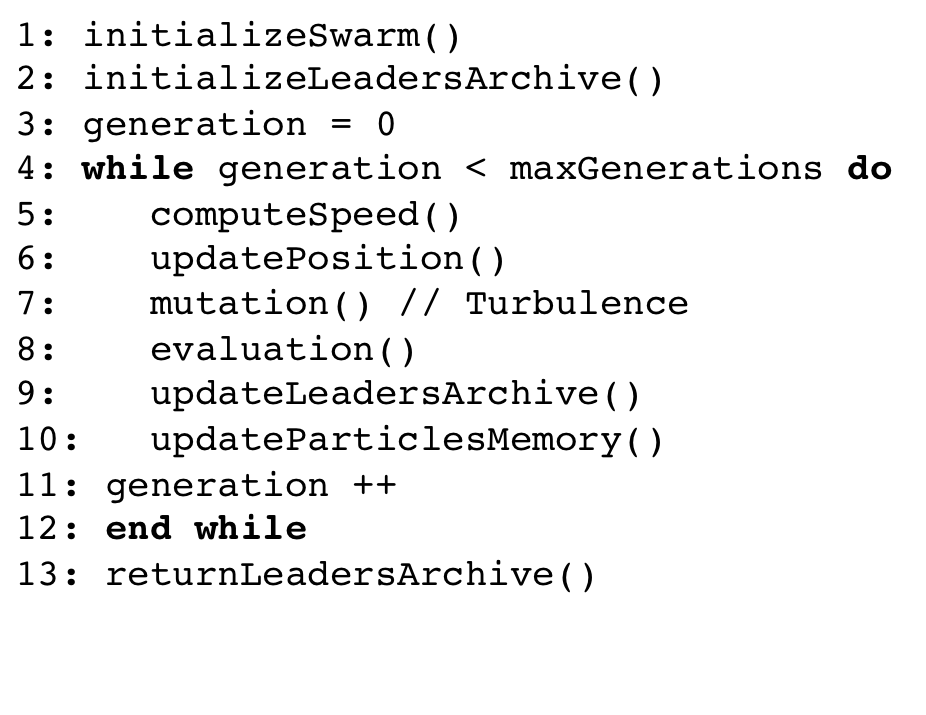
\includegraphics[width=\linewidth]{images/bab4/smpso_code.png}
        \caption{ Pseudocode Controller untuk Menampilkan Antarmuka A }
        \label{pdm}
      \end{figure}
      
    \subsection{Antarmuka Halaman B}
    Penjelasan otorisasi terhadap antarmuka B, link yang tersedia dalam antarmuka B, dan penjelasan \textit{exception} jika terjadi masalah baik otorisasi ataupun autentikasi saat mengakses antarmuka ini.
  
      \begin{figure}[H]
        \centering
        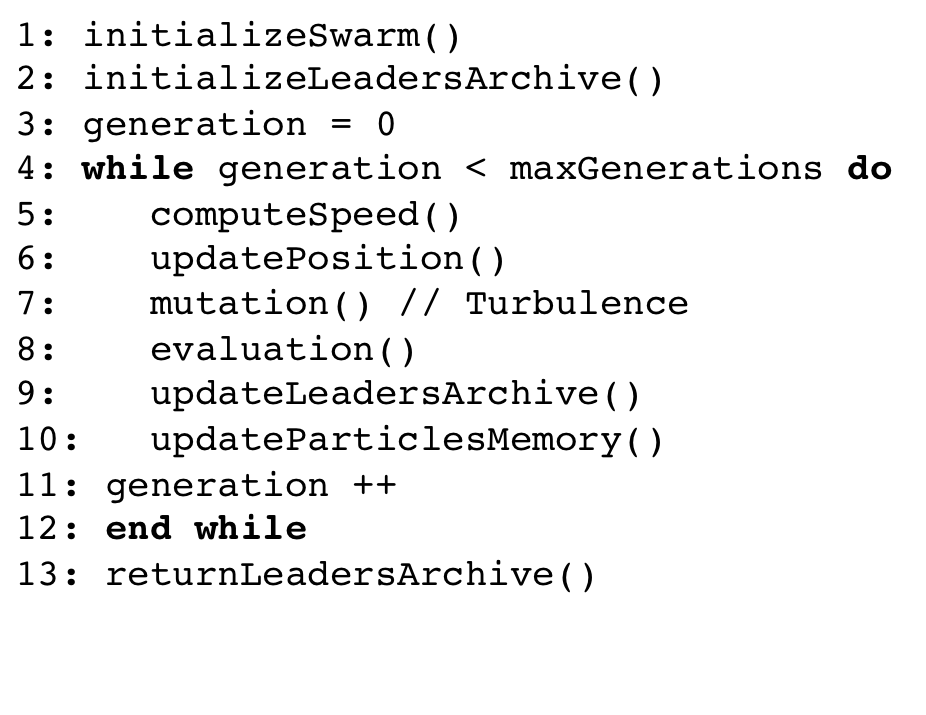
\includegraphics[width=\linewidth]{images/bab4/smpso_code.png}
        \caption{ Pseudocode Controller untuk Menampilkan Antarmuka B }
        \label{pdm}
      \end{figure}
    
    
\section{Pemasangan Proyek}
	Pembangunan dilakukan secara online, dan tersebar (tidak hanya menggunakan satu \textit{service provider} saja.
    Berikut dijelaskan langkah-langkah pembangunan proyek:
    
    \subsection{Konfigurasi Domain}
    Domain yang dipilih berasal dari Namecheap.com , dengan langkah-langkah konfigurasi sebagai berikut :
    \begin{enumerate}
    \item Langkah 1
    \item Langkah 2
    \end{enumerate}
    \subsection{Konfigurasi VPS}
    Domain yang dipilih berasal dari DigitalOcean dan Google Cloud Computing , dengan langkah-langkah konfigurasi sebagai berikut :
    \begin{enumerate}
    \item DigitalOcean
      \begin{enumerate}
      \item Langkah 1
      \item Langkah 2
      \end{enumerate}
    \item Google Cloud Computing
      \begin{enumerate}
      \item Langkah 1
      \item Langkah 2
      \end{enumerate}
    \end{enumerate}
    
    \subsection{Konfigurasi PostgreSQL}
    PostgreSQL diinstal dalam VPS, dengan langkah-langkah konfigurasi sebagai berikut :
    \begin{enumerate}
    \item Langkah 1
    \item Langkah 2
    \end{enumerate}
    
    \subsection{Konfigurasi Node.js}
    Node.js diinstall dalam VPS, dengan langkah-langkah konfigurasi sebagai berikut :
    \begin{enumerate}
    \item Langkah 1
    \item Langkah 2
    \end{enumerate}
    
    \subsection{Konfigurasi MongoDB}
    MongoDB diinstall dalam VPS, dengan langkah-langkah konfigurasi sebagai berikut :
    \begin{enumerate}
    \item Langkah 1
    \item Langkah 2
    \end{enumerate}
    
    \subsection{Konfigurasi SMTP Service}
    SMTP \textit{service} yang digunakan berasal dari sendgrid.net, dengan langkah-langkah konfigurasi sebagai berikut :
    \begin{enumerate}
    \item Langkah 1
    \item Langkah 2
    \end{enumerate}
